\subsection{Feature extraction}

Any input to a neural network can contain a lot of different information.
The information is built from a series of (possibly recurring) objects, that may be arbitrarily scattered across the input.
These objects determine the meaning of the input.

In the case of images, features exist on multiple abstractions.
When completely zooming in, one pixel tells a very local story.
A group of pixels may tell the story of a single object.
Sets of groups model the interaction between objects.
Lastly, combining all sets results in the full image.

Similar to masking, it is useful to extract as much information as possible into a smaller image representation: a feature vector.
A feature extractor that creates feature vectors from images can be trained using various algorithms.

One algorithm to train a feature extractor is a simple framework for contrastive learning of visual representations (SimCLR)~\cite{Chen2020}.
SimCLR learns features by augmenting the same data twice and maximizing the agreement between the representations of those augmentations.
No targets are needed.
SimCLR is self-supervised.

The original image $\vec{x}$ is transformed twice with transform $t$ and $t' \sim T$ to create $\tilde{\vec{x}}_{i,j}$.
Any transformation can be sampled from transformation space $T$, but the original authors experiment with cropping, resizing, flipping, color dropping, and color jittering among others.
Then, with a chosen convolutional neural network backbone $f$, the transformed images are encoded in representations $\vec{h}_{i,j}$.
The representations are then projected with a projection head $g$ to a space in which the loss function between the resulting $\vec{z}_{i,j}$ is calculated.
The loss function is typically the normalized-temperature cross-entropy loss (NT-Xent) and is defined as
\begin{align}
    \text{NT-Xent} = - \log \frac{\exp(s_{i,j} / \tau)}{\sum_{k=1}^{2N}\mathbb{1}_{[k\neq i]}\exp(s_{i,j} / \tau)},
\end{align}
where $s_{i,j}$ is the similarity
\begin{align}
    s_{i,j} = \frac{\vec{z}_i \cdot \vec{z}_j }{\|\vec{z}_i\|\|\vec{z}_j\|},
\end{align}
$N$ the number of samples in the batch, $\tau$ the temperature to scale the similarity with, and $\mathbb{1}$ the indicator function which maps all elements that satisfy it subscript to 1.
SimCLR is visualized in \cref{fig:simclr}.


\begin{figure}
    \centering
    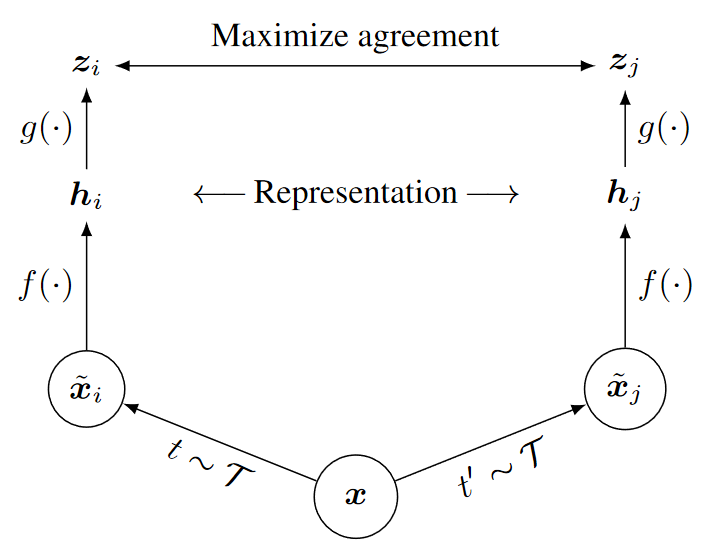
\includegraphics[width=\linewidth]{pediatric-brain-tumours/images/simclr.png}
    \caption[SimCLR]{
        A simple framework for contrastive learning of visual representations.
        Two augmentations of an image are encoded into feature vectors before being projected into a space where a contrastive loss is calculated.
        Learned feature extractor $f$ encodes images into $\vec{h}$ for downstream tasks.
        Reproduced from \fullcite{Chen2020} (Ref.~\cite{Chen2020}).
    }
    \label{fig:simclr}
\end{figure}

A SimCLR trained backbone can then be used as a compression algorithm adapted to the domain it has been trained on.
